\documentclass[12pt,a4paper]{article}

\usepackage[a4paper,margin=1in]{geometry}
\usepackage{graphicx}
\usepackage{booktabs}
\usepackage{amsmath,amssymb}
\usepackage{float}
\usepackage{hyperref}
\usepackage{xurl}
\usepackage{xcolor}
\usepackage{listings}
\usepackage{enumitem}
\usepackage{fancyhdr}
\usepackage{longtable}

\hypersetup{colorlinks=true,linkcolor=blue,urlcolor=blue}

\pagestyle{fancy}
\fancyhf{}
\lhead{ICS1512}
\rhead{Machine Learning Algorithms Laboratory}
\cfoot{\thepage}

\setlength{\parskip}{0.4em}
\setlength{\parindent}{0pt}
\setlength{\headheight}{15pt}

\setlength{\floatsep}{10pt plus 2pt minus 2pt}
\setlength{\textfloatsep}{12pt plus 2pt minus 2pt}
\setlength{\intextsep}{10pt plus 2pt minus 2pt}

\setcounter{topnumber}{3}
\setcounter{bottomnumber}{3}
\setcounter{totalnumber}{4}
\renewcommand{\topfraction}{0.85}
\renewcommand{\bottomfraction}{0.85}
\renewcommand{\textfraction}{0.15}
\renewcommand{\floatpagefraction}{0.8}

\lstset{
language=Python,
basicstyle=\ttfamily\small,
numbers=left,
frame=single,
breaklines=true,
showstringspaces=false
}

\begin{document}

\begin{tabular}{|p{4cm}|p{11cm}|}
\hline
Experiment No. & 1 \\ \hline
Experiment Title & Working with Python Packages: NumPy, SciPy, Scikit-Learn, Matplotlib, and Pandas (Iris Botanical Dataset) \\ \hline
Student Name & Srinivasan M \\ \hline
Register Number & 3122247001063 \\ \hline
Faculty & Dr. Poreddy Ajay Kumar Reddy \\ \hline
Submission Date & \today \\ \hline
\end{tabular}

\vspace{0.3cm}

\section{Objective}
The main goals of this exploratory analysis on the Iris dataset are:
\begin{itemize}[noitemsep]
    \item Leverage core Python numerical packages (NumPy, Pandas, Seaborn, Matplotlib) to perform automated statistical profiling on botanical morphometric features.
    \item Evaluate multi-dimensional linear separability between target species (Setosa, Versicolor, Virginica).
    \item Export diagnostic visual figures into \texttt{figures\_iris/}.
\end{itemize}

\section{Problem Statement}
In supervised classification tasks, identifying attribute pairs that achieve clean hyper-planar separability significantly improves model training speed and accuracy. Manual feature plotting for multi-class targets can be tedious. This report uses an automated EDA pipeline to evaluate class overlap and feature correlation bounds across all four morphometric measurements of the Iris dataset.

\section{Dataset Description}
The **Iris Botanical Dataset** consists of 150 flower samples evenly divided across three species.

\begin{longtable}{|p{6cm}|p{8cm}|}
\hline
Dataset Name & Iris Botanical Dataset \\ \hline
Dataset Source & UCI Machine Learning Repository \\ \hline
Number of Samples & 150 (50 per species class) \\ \hline
Number of Features & 4 continuous numerical dimensions \\ \hline
Number of Classes & 3 (Iris-setosa, Iris-versicolor, Iris-virginica) \\ \hline
Missing Values & 0 missing records \\ \hline
Train-Test Split & N/A (Exploratory Analysis Phase) \\ \hline
\end{longtable}

The dataset attributes include:
\begin{itemize}[noitemsep]
    \item \texttt{SepalLengthCm}: Sepal length in centimeters.
    \item \texttt{SepalWidthCm}: Sepal width in centimeters.
    \item \texttt{PetalLengthCm}: Petal length in centimeters.
    \item \texttt{PetalWidthCm}: Petal width in centimeters.
    \item \texttt{Species}: Iris species category (Target).
\end{itemize}

\section{Exploratory Data Analysis}
The automated EDA module generated 17 visualizations saved in \texttt{figures\_iris/}.

\subsection{Histograms of Numerical Features}

\begin{figure}[H]
\centering
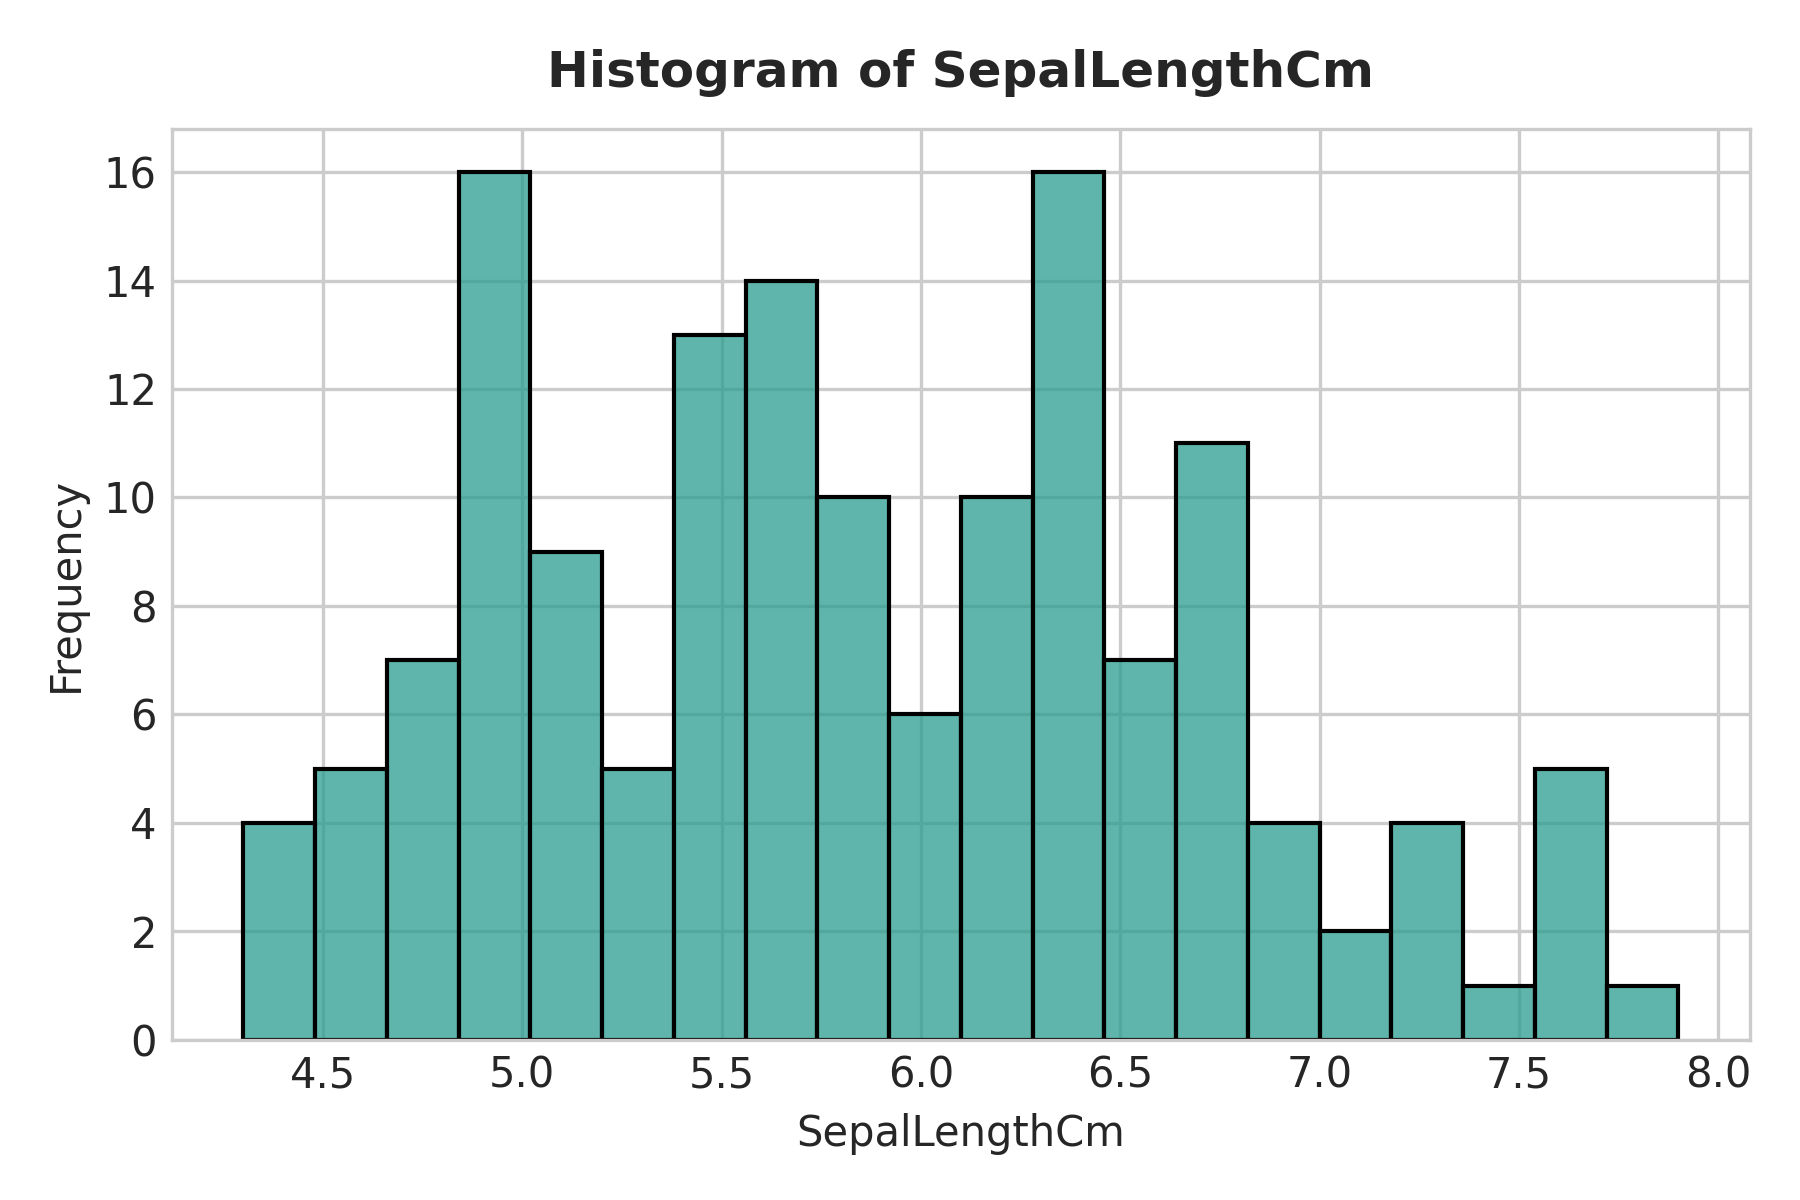
\includegraphics[width=0.75\linewidth]{figures_iris/hist_SepalLengthCm.png}
\caption{Histogram of Sepal Length}
\label{fig:iris_hist_sepal_len}
\end{figure}
\textbf{Inference:} Sepal length ranges from 4.3 cm to 7.9 cm, forming a unimodal distribution centered near 5.8 cm.

\begin{figure}[H]
\centering
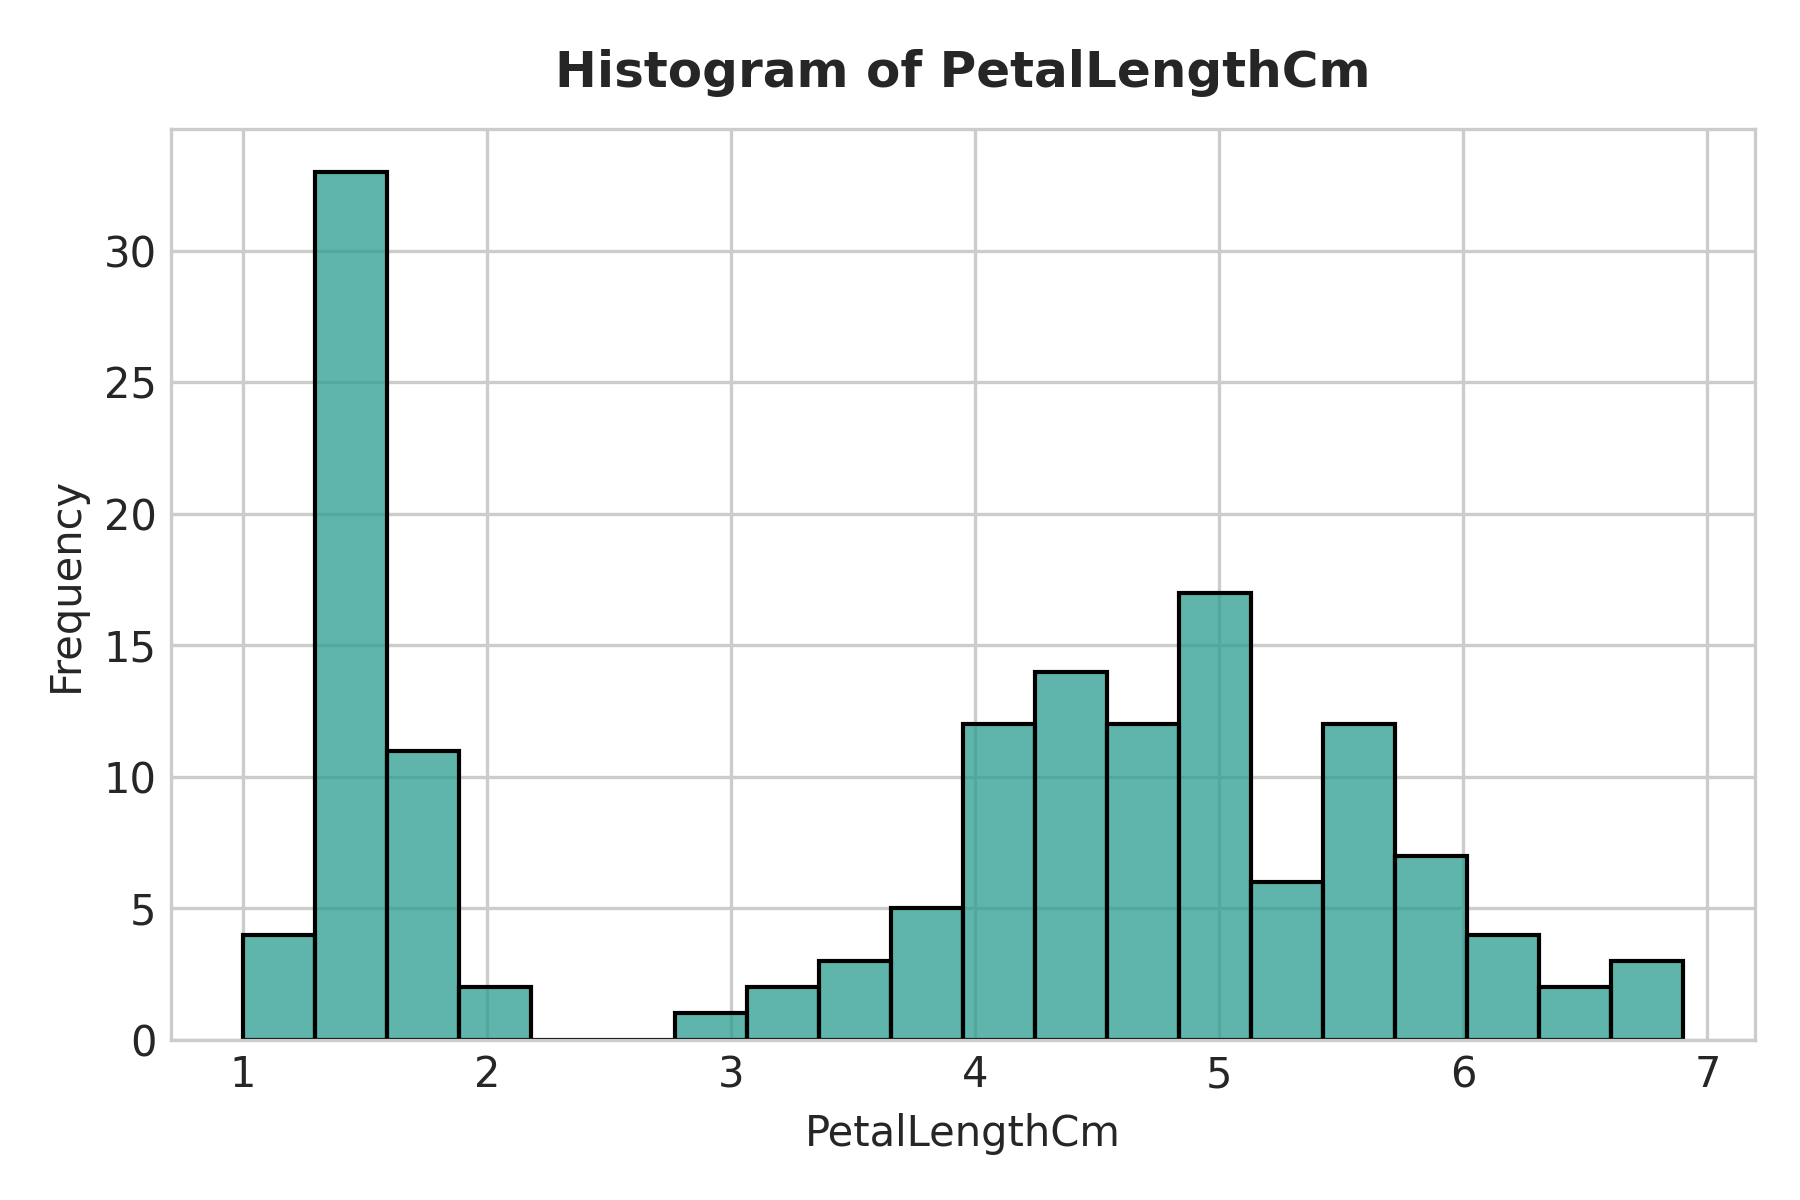
\includegraphics[width=0.75\linewidth]{figures_iris/hist_PetalLengthCm.png}
\caption{Histogram of Petal Length}
\label{fig:iris_hist_petal_len}
\end{figure}
\textbf{Inference:} Petal length shows a distinct bimodal distribution with a clear density gap between 2.0 cm and 3.0 cm, isolating Iris-setosa from Versicolor and Virginica.

\subsection{Box Plots of Numerical Features}

\begin{figure}[H]
\centering
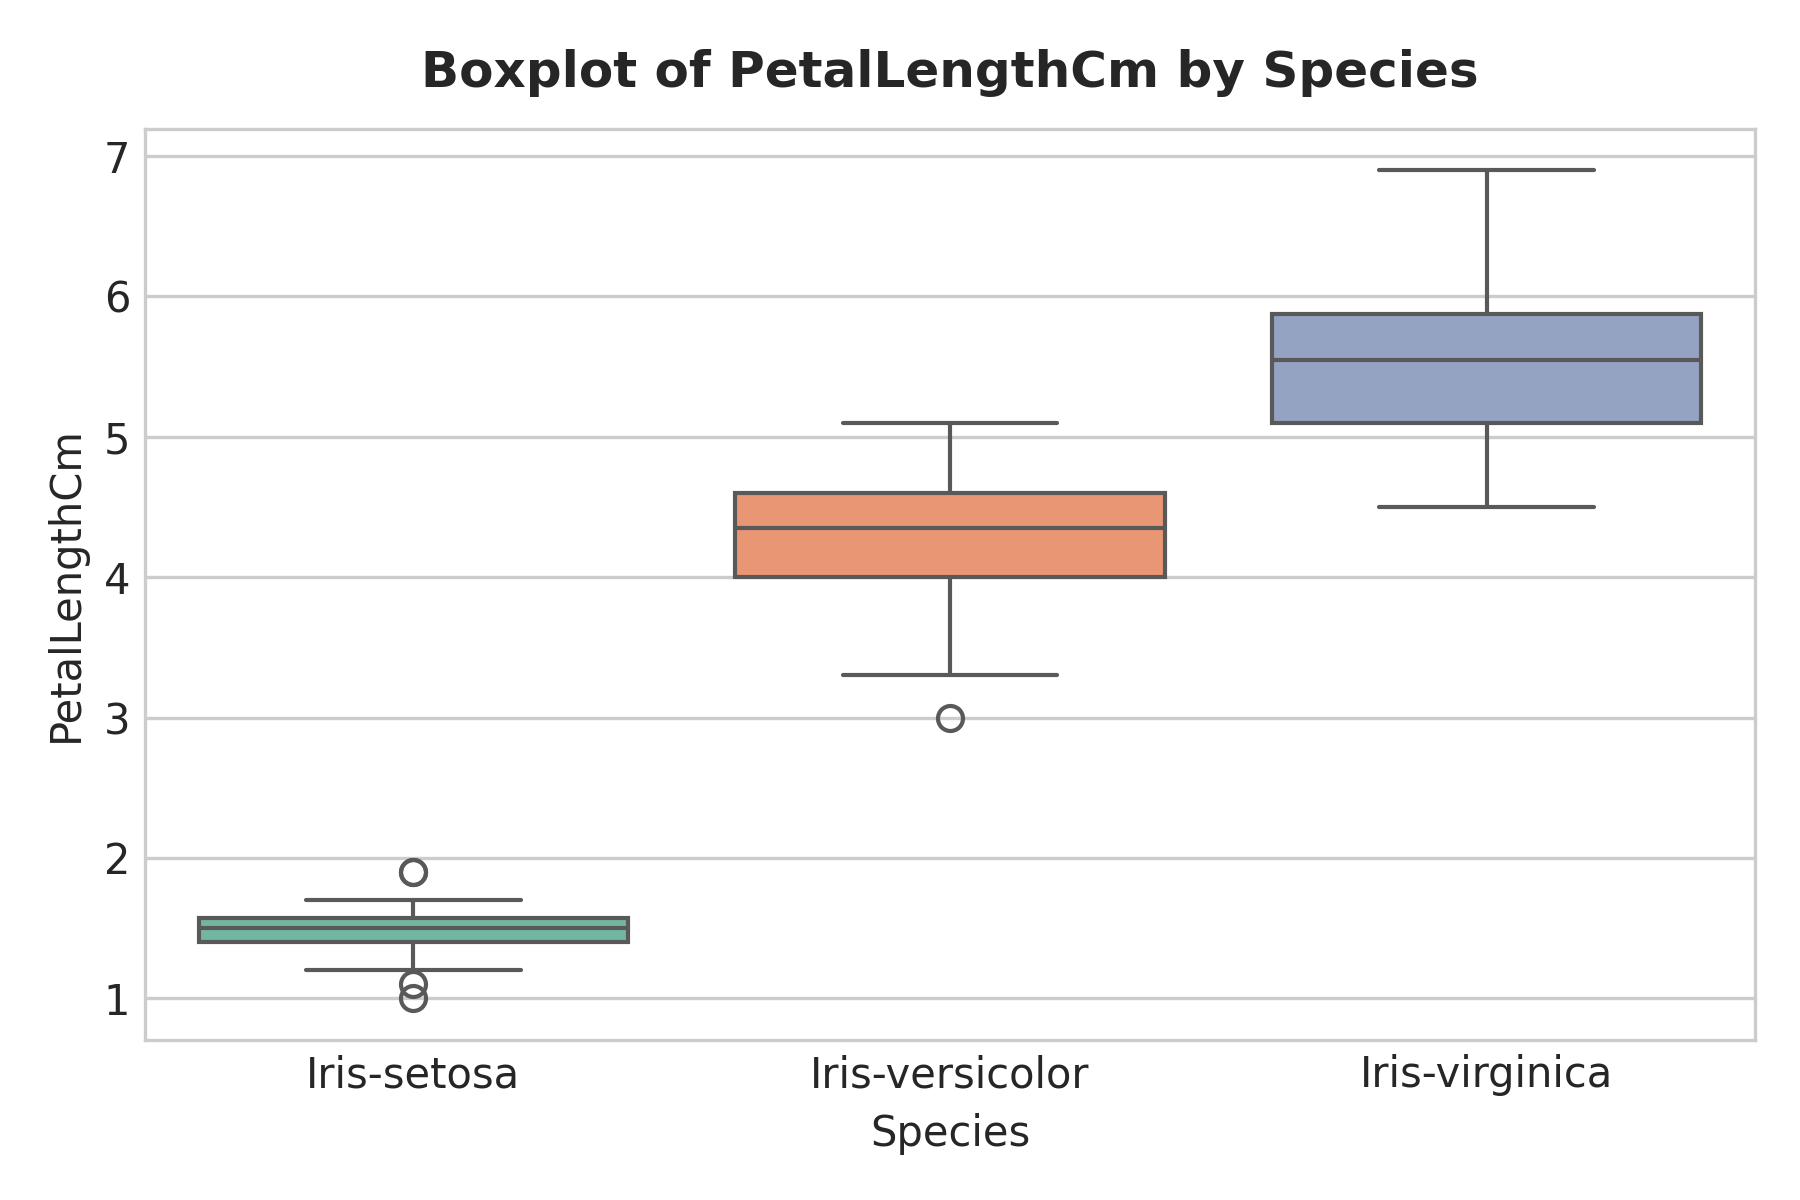
\includegraphics[width=0.75\linewidth]{figures_iris/box_PetalLengthCm.png}
\caption{Box Plot of Petal Length by Species}
\label{fig:iris_box_petal_len}
\end{figure}
\textbf{Inference:} Iris-setosa features significantly shorter petals (1.0--1.9 cm) with non-overlapping interquartile ranges relative to Versicolor (3.0--5.1 cm) and Virginica (4.5--6.9 cm).

\subsection{Kernel Density Estimation (KDE) Plots}

\begin{figure}[H]
\centering
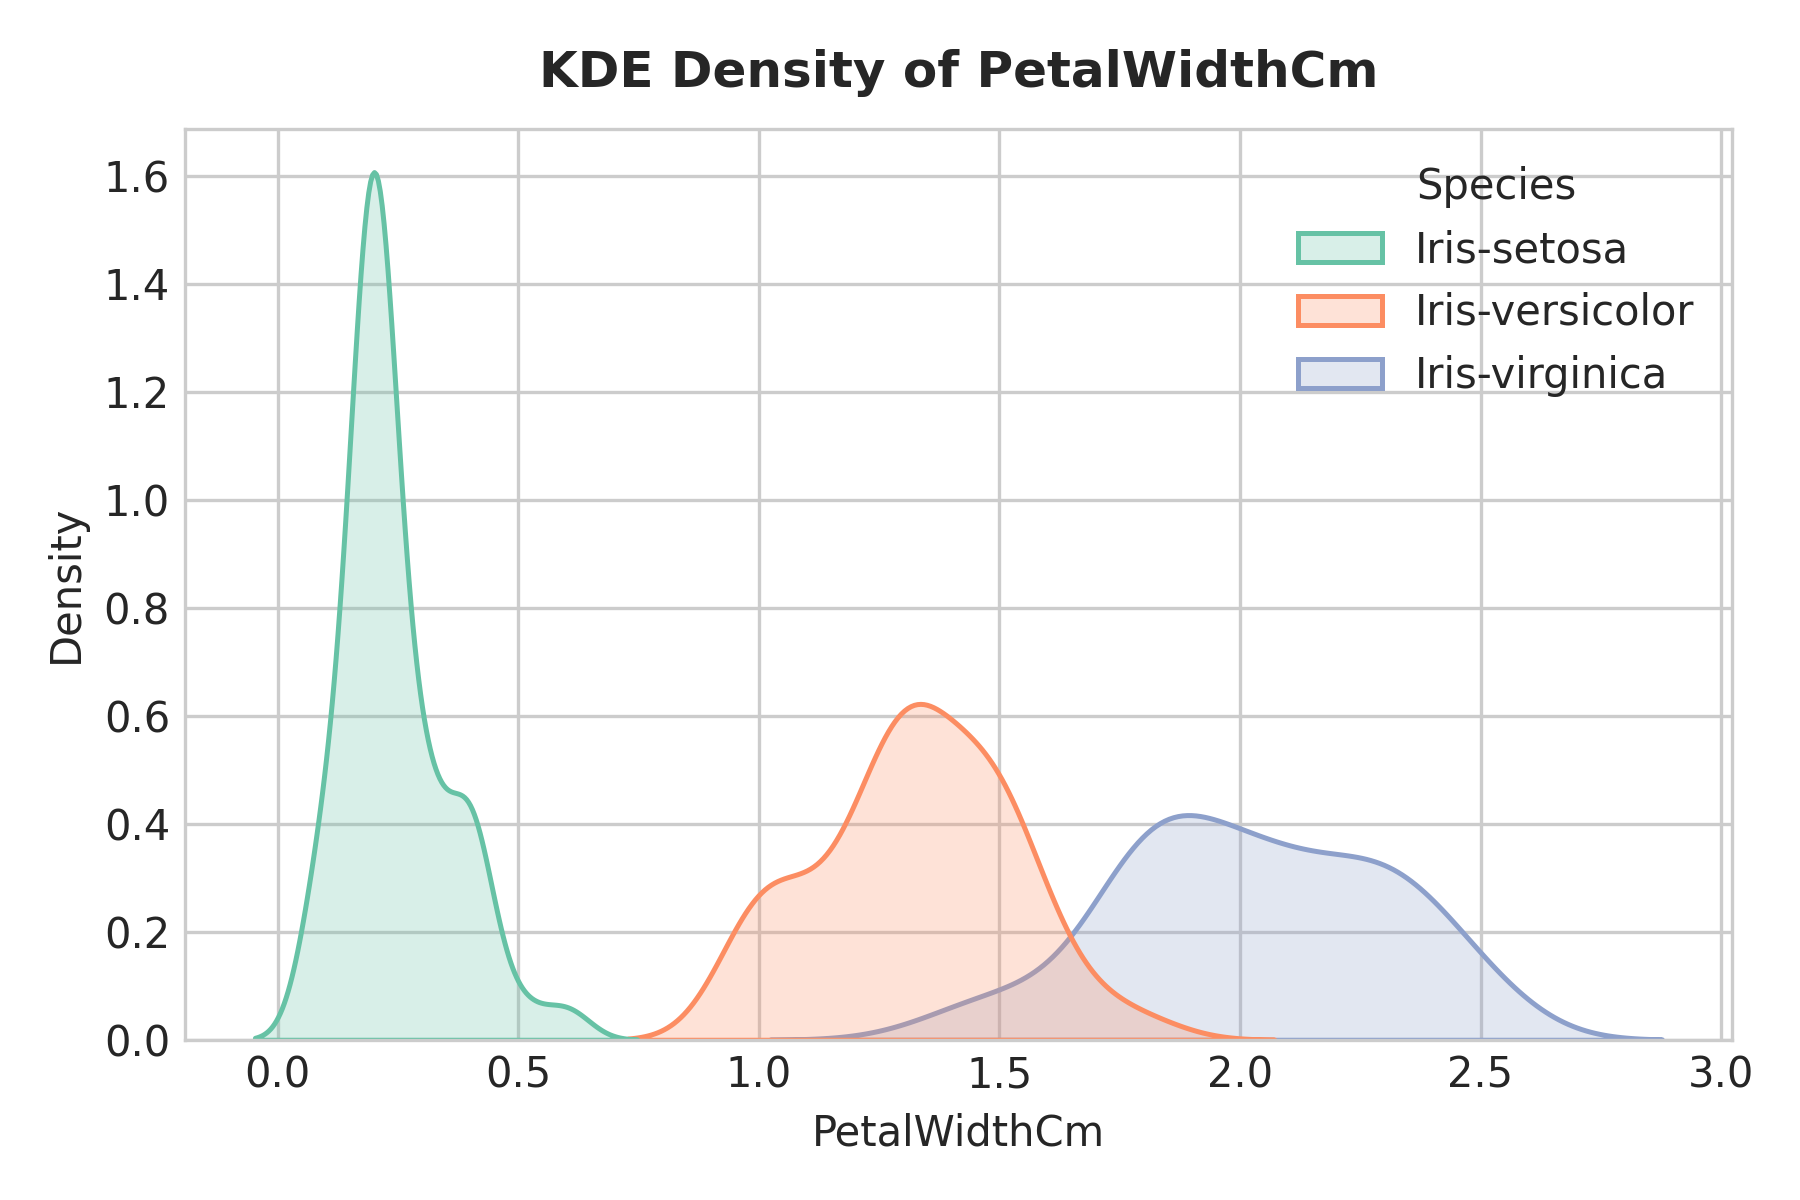
\includegraphics[width=0.75\linewidth]{figures_iris/kde_PetalWidthCm.png}
\caption{KDE Density of Petal Width by Species}
\label{fig:iris_kde_petal_width}
\end{figure}
\textbf{Inference:} Density estimation highlights complete linear separability of Setosa along petal width, while Versicolor and Virginica display partial overlap in the 1.4--1.8 cm interval.

\subsection{Count Plots of Categorical Features}

\begin{figure}[H]
\centering
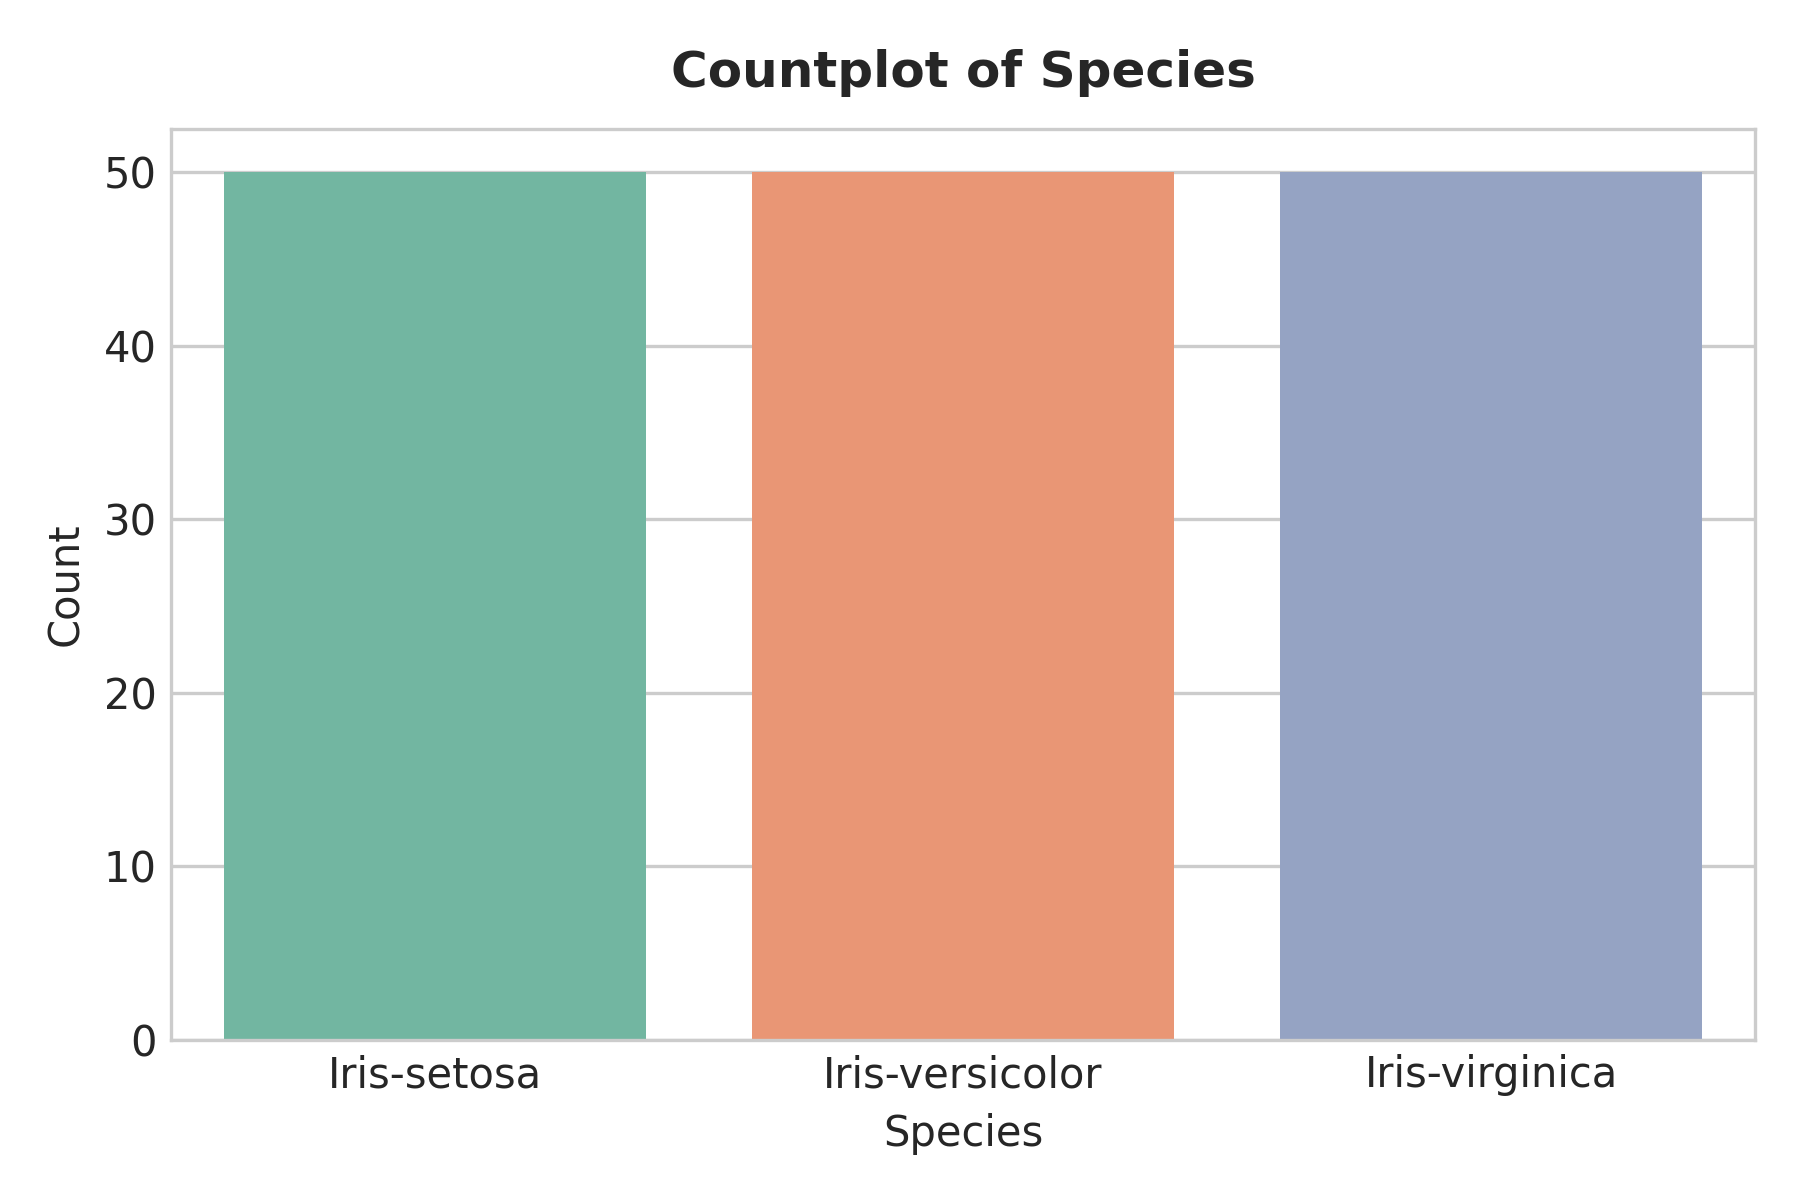
\includegraphics[width=0.75\linewidth]{figures_iris/count_Species.png}
\caption{Count Plot of Iris Species}
\label{fig:iris_count_species}
\end{figure}
\textbf{Inference:} Displays a perfectly balanced dataset containing exactly 50 samples for each species class.

\subsection{Correlation Heatmap of Numerical Features}

\begin{figure}[H]
\centering

\includegraphics[width=0.75\linewidth]{figures_iris/correlation_heatmap.png}
\caption{Correlation Heatmap of Iris Features}
\label{fig:iris_correlation_heatmap}
\end{figure}
\textbf{Inference:} Petal length and petal width display a high positive correlation ($r = 0.96$). Sepal length also correlates strongly with petal dimensions ($r > 0.81$).

\subsection{Pairwise Scatter Matrix (Pair Plot)}

\begin{figure}[H]
\centering

\includegraphics[width=0.75\linewidth]{figures_iris/pairplot.png}
\caption{Pair Plot of Iris Features by Species}
\label{fig:iris_pairplot}
\end{figure}
\textbf{Inference:} The pairplot grid visually confirms that Setosa forms a linearly isolated cluster in every bivariate projection, whereas Versicolor and Virginica require non-linear or multi-feature boundaries.

\subsection{Bivariate Scatter Plots}

\begin{figure}[H]
\centering
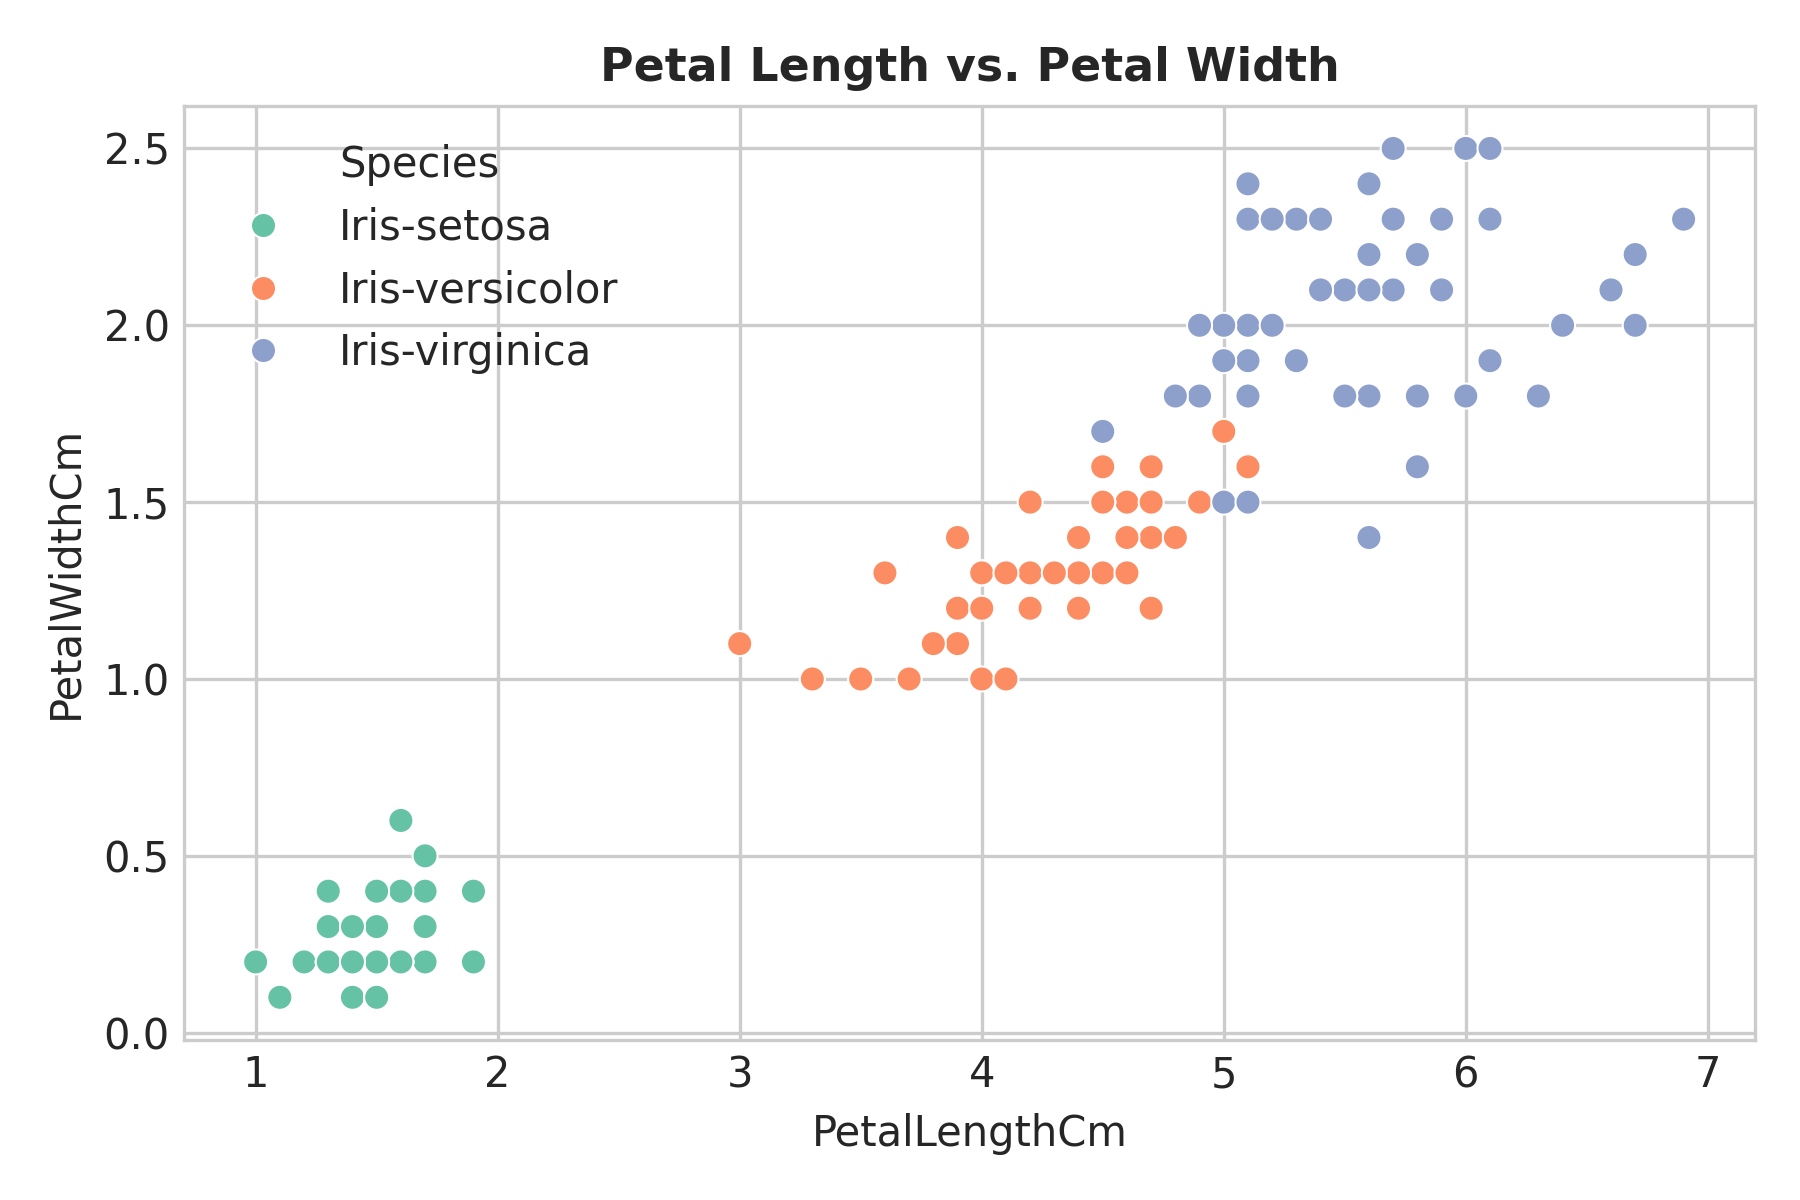
\includegraphics[width=0.75\linewidth]{figures_iris/scatter_PetalLength_vs_PetalWidth.png}
\caption{Scatter Plot: Petal Length vs. Petal Width}
\label{fig:iris_scatter_petal}
\end{figure}
\textbf{Inference:} Displays strong linear clustering per species, confirming petal dimensions as the dominant discriminative feature pair.

\section{Data Preprocessing}
The Iris dataset contains zero missing values and zero duplicate samples. Feature standardization using Z-score scaling ($z = \frac{x - \mu}{\sigma}$) is recommended prior to training distance-sensitive algorithms like K-Nearest Neighbors (KNN) or Support Vector Machines (SVM).

\section{Machine Learning Algorithms}
\begin{itemize}[noitemsep]
    \item \textbf{Suitable Models}: Decision Trees, Random Forests, Support Vector Machines (RBF/Linear kernel), K-Nearest Neighbors (KNN).
    \item \textbf{Feature Selection}: ANOVA F-test via \texttt{SelectKBest} or Principal Component Analysis (PCA) for dimensionality reduction.
\end{itemize}

\section{Experimental Setup}
Executed on Python 3.10+ using Pandas, NumPy, Matplotlib, and Seaborn on Windows 11.

\section{Hyperparameter Selection}
Density kernel bandwidths and pairwise bin sizing were determined dynamically using Seaborn defaults.

\section{Results}
All 17 visualization outputs were successfully generated and stored in \texttt{figures\_iris/}.

\section{Result Visualization}
The visualizations demonstrate that petal dimensions (\texttt{PetalLengthCm} and \texttt{PetalWidthCm}) provide clean multi-class discrimination boundaries.

\section{Discussion}
The Iris dataset provides a foundational benchmark for multiclass linear vs. non-linear decision boundaries.
\begin{itemize}[noitemsep]
    \item \textbf{Strengths}: Small dimension, balanced classes, zero null values.
    \item \textbf{Insights}: Setosa requires only simple threshold rules, whereas Virginica and Versicolor require soft-margin classifiers.
\end{itemize}

\section{Conclusion}
The automated EDA framework effectively characterized the Iris dataset, establishing that petal length and width serve as optimal predictive attributes for species classification.

\section{References}
\begin{enumerate}[label={[\arabic*]}, leftmargin=2em]
    \item Fisher, R. A., ``The use of multiple measurements in taxonomic problems,'' *Annals of Eugenics*, 1936.
    \item UCI Machine Learning Repository, ``Iris Dataset,'' \url{https://archive.ics.uci.edu/ml/datasets/iris}.
\end{enumerate}

\end{document}
